\documentclass[a4paper]{article}
\usepackage[a4paper,top=2cm,bottom=2cm,left=1cm,right=1cm,marginparwidth=1.75cm]{geometry}
% \usepackage[spanish]{babel}
% \selectlanguage{spanish}
% \usepackage[utf8]{inputenc}
% \usepackage[T1]{fontenc}
% \usepackage[spanish]{babel}

% \usepackage[T1]{fontenc}
\usepackage{graphicx} %Paquete para usar imagenes
\usepackage{listings}
\usepackage{xcolor}
\usepackage{tcolorbox}

\definecolor{background}{HTML}{E7EBF4}
\definecolor{bg}{HTML}{1a1b26}
\definecolor{fg}{HTML}{a9b1d6}
\definecolor{comment}{HTML}{848cb5}
\definecolor{cyan}{HTML}{82aaff}
\definecolor{orange}{HTML}{ff9e64}
\definecolor{yellow}{HTML}{e9d78e}
\definecolor{purple}{HTML}{c792ea}
\definecolor{green}{HTML}{7fdbca}
\definecolor{numbers}{HTML}{9854f1}
\definecolor{keyword}{HTML}{9854f1}

\lstset{
    showspaces=false, % Evita mostrar espacios en blanco como ␣
    showstringspaces=false,
    inputencoding=utf8,
    extendedchars=true,
    literate=%
    {á}{{\'a}}1
    {é}{{\'e}}1
    {í}{{\'i}}1
    {ó}{{\'o}}1
    {ú}{{\'u}}1
    {ñ}{{\~n}}1
}
\lstdefinestyle{mystyle}{
    language=Python,
    basicstyle=\ttfamily,
    keywordstyle=\color{keyword},
    commentstyle=\color{comment},
    numbers=none,
    numberstyle=\tiny\color{numbers},
    frame=none,
    breaklines=true,
    % showstringspaces=false
    xleftmargin=0mm,
    xrightmargin=0mm,
}

\lstset{style=mystyle}

\newtcolorbox{mycodebox}[1][]{
    arc=7pt,  % Radio de las esquinas redondeadas
    colback=background,  % Color de fondo del cuadro
    boxrule=0.5pt,  % Grosor de la línea del cuadro
    colframe=background,
    width=0.8\textwidth,   % Anchura del cuadro
    % height=5cm,            % Altura del cuadro
    % breakable,
    #1  % Otras opciones personalizadas que puedas necesitar
}


\newtcolorbox{mycodeboxl}[1][]{
    arc=7pt,  % Radio de las esquinas redondeadas
    colback=background,  % Color de fondo del cuadro
    boxrule=0.5pt,  % Grosor de la línea del cuadro
    colframe=background,
    width=0.94\textwidth,   % Anchura del cuadro
    % height=5cm,            % Altura del cuadro
    % breakable,
    #1  % Otras opciones personalizadas que puedas necesitar
}

% Documento
\begin{document}
\newgeometry{left=3cm,right=3cm,top=2cm,bottom=2cm}
\begin{titlepage}

%--------------- Nuevo comendo de linea ----------------->
\newcommand{\linea}{\rule{\linewidth}{0.7mm}} 
\center
%--------------- Universidad, facultad y carrera ----------------->
\textbf{\Large UNIVERSIDAD NACIONAL DE SAN ANTONIO ABAD DEL CUSCO}\\[0.2cm]
\textbf{\Large FACULTAD DE INGENIERÍA ELÉCTRICA, ELECTRÓNICA,INFORMÁTICA Y MECÁNICA}\\[0.2cm]
\textbf{\Large INGENIERÍA INFORMÁTICA Y DE SISTEMAS\\[0.6cm]}

%--------------- Escudos png ----------------->

\includegraphics[width=8cm]{src/escudo-unsaac.png}
\vfill

%--------------- Tema ----------------->
\linea
\\[0.3cm]
% \vfill
\textbf{\LARGE Guía de Laboratorio 2 - Algoritmos de Generación de Circunferencias}\\[0.2cm]
\linea \\
\vfill

%--------------- Integrantes ----------------->
\textit{\Large Alumno:}\\
%Integrantes del grupo
    \textbf{\large Ian Logan Will Quispe Ventura}\\
    \textit{211359}\\
    % \vfill

%--------------- Profesor y curso ----------------->
\vspace{0.3cm}
    \textit{\Large Docente:}\\
    \textbf{\large Hector Eduardo Ugarte Rojas}\\
\vspace{0.5cm}
    \textit{\Large Curso:}\\
    \textbf{\large Computación Gráfica}\\
    \vfill

\vspace{0.4cm}
    \textbf{\Large Cusco - Perú }\\
    \textbf{\large 2023 - II }\\
    \newpage
    \end{titlepage}

\restoregeometry
\newpage
% •·•·•·•·•·•••·•·•·•·•·•·•·•·•·•·•·•·•·•·•·•·•·•·•·•·•.,..,
% \section{Funcionamiento del algoritmo DDA}
\Large{\textbf{Funcionamiento del algoritmo de 2 Vías}}\\[0.5cm]
Modulo Display 
\begin{center}
\begin{mycodebox}
\begin{lstlisting}
def display_2vias():
    glClear(GL_COLOR_BUFFER_BIT)
    glPointSize (1)
    glColor3f(0.5, 0.3, 0.9) 
    circulo2vias(150, 250, 100)
    circulo2vias(350, 250, 100)
    circulo2vias(250, 350, 100)
    circulo2vias(250, 150, 100)
    glFlush()
\end{lstlisting}
\end{mycodebox}
\end{center}
% \newpage
Gráfico generado
\begin{center}
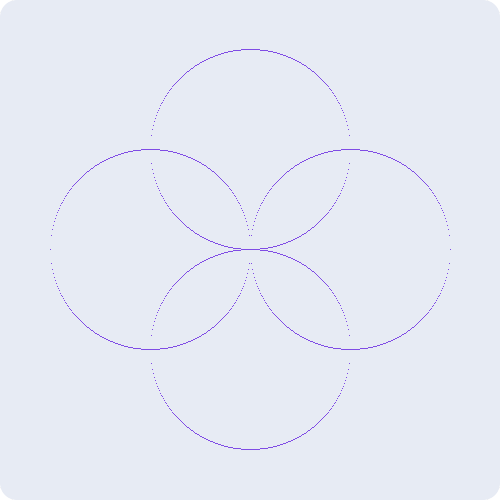
\includegraphics[width=15cm]{src/2vias.png}
\end{center}
\newpage
% \newpage

\Large{\textbf{Funcionamiento del algoritmo de 4 Vías}}\\[0.5cm]
Modulo Display 
\begin{center}
\begin{mycodebox}
\begin{lstlisting}
def display_4vias():
    glClear(GL_COLOR_BUFFER_BIT)
    glPointSize (1)
    glColor3f(0.5, 0.3, 0.9) 
    circulo4vias(150, 250, 100)
    circulo4vias(350, 250, 100)
    circulo4vias(250, 350, 100)
    circulo4vias(250, 150, 100)
    glFlush()
\end{lstlisting}
\end{mycodebox}
\end{center}
Gráfico generado
\begin{center}
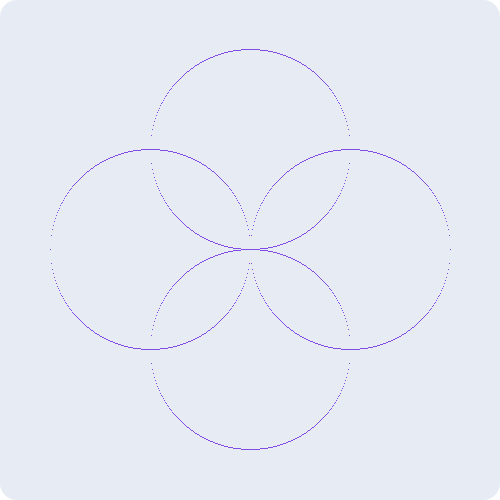
\includegraphics[width=15cm]{src/4vias.png}
\end{center}
\newpage

\Large{\textbf{Funcionamiento del algoritmo de 8 vías}}\\[0.5cm]
Modulo Display 
\begin{center}
\begin{mycodebox}
\begin{lstlisting}
def display_8vias():
    glClear(GL_COLOR_BUFFER_BIT)
    glPointSize (1)
    glColor3f(0.5, 0.3, 0.9) 
    circulo8vias(150, 250, 100)
    circulo8vias(350, 250, 100)
    circulo8vias(250, 350, 100)
    circulo8vias(250, 150, 100)
    glFlush()
\end{lstlisting}
\end{mycodebox}
\end{center}
Gráfico generado
\begin{center}
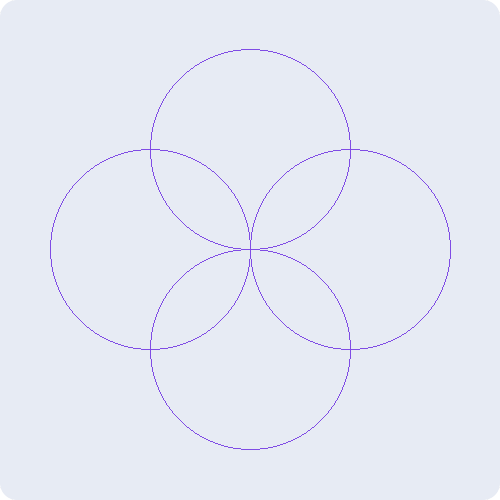
\includegraphics[width=15cm]{src/8vias.png}\\
\end{center}
\newpage

\Large{\textbf{Funcionamiento del algoritmo de Punto Medio}}\\[0.5cm]
Modulo Display 
\begin{center}
\begin{mycodebox}
\begin{lstlisting}
def display_PtoMedio():
    glClear(GL_COLOR_BUFFER_BIT)
    glPointSize (1)
    glColor3f(0.5, 0.3, 0.9) 
    circuloPtoMEdio(150, 250, 100)
    circuloPtoMEdio(350, 250, 100)
    circuloPtoMEdio(250, 350, 100)
    circuloPtoMEdio(250, 150, 100)
    glFlush()
\end{lstlisting}
\end{mycodebox}
\end{center}
Gráfico generado
\begin{center}
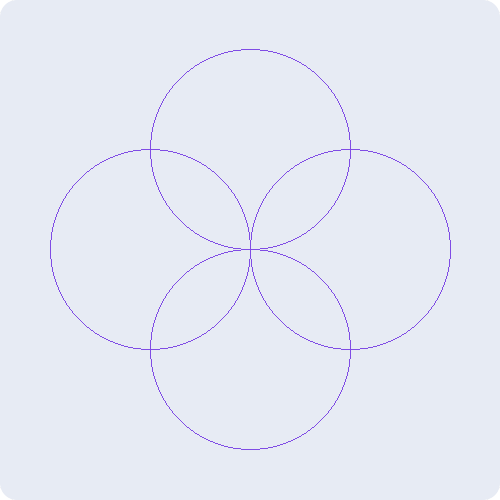
\includegraphics[width=15cm]{src/ProMedioCir.png}\\
\end{center}
\newpage

\Large{\textbf{Funcionamiento del algoritmo de trazados de lineas y círculo}}\\[0.5cm]
Necesitamos un módulo que dibuje y ejecute las lineas mediante el módulo DDA 
\begin{center}
\begin{mycodeboxl}
\begin{lstlisting}
def lineas(x0, y0, r, n_puntos):
    # Calcularemos el ángulo inicial de la primera linea
    angulo_inicial = 360 / n_puntos
    puntos_interseccion = []

    for i in range(n_puntos):
        # El ángulo incrementará a cada linea que se quiera dibujar 
        angulo = i * angulo_inicial
        # Calcularemos los puntos que intersectan con la circunferencia
        angulo_radianes = math.radians(angulo)
        x = x0 + r * math.cos(angulo_radianes)
        y = y0 + r * math.sin(angulo_radianes)

        #Dibujar las lineas desde el origen hasta un punto de la circunferencia
        DDA(x0, y0, int(x), int(y)) 
        # Los puntos se duardan para luego unirlos formando un polígono
        puntos_interseccion.append((x, y))

    for a in range(n_puntos):
        # Conenctar las anteriores lineas para formar un polígono regular (dodecágono) 
        # (a + 1) % n_puntos Permite unir el punto final con el inicial
        DDA(int(puntos_interseccion[a][0]), int(puntos_interseccion[a][1]), int(puntos_interseccion[(a + 1) % n_puntos][0]), int(puntos_interseccion[(a + 1) % n_puntos][1]))
\end{lstlisting}
\end{mycodeboxl}
\end{center}
\newpage
Módulo display que ejecutará el algoritmo Punto Medio y el de las lineas
\begin{center}
\begin{mycodebox}
\begin{lstlisting}
def display():
    glClear(GL_COLOR_BUFFER_BIT)
    circuloPtoMEdio(250, 250, 150)
    glColor3f(0.5, 0.3, 0.9) 
    lineas(250, 250, 150, 12)
    glFlush()
\end{lstlisting}
\end{mycodebox}
\end{center}
Gráfico generado
\begin{center}
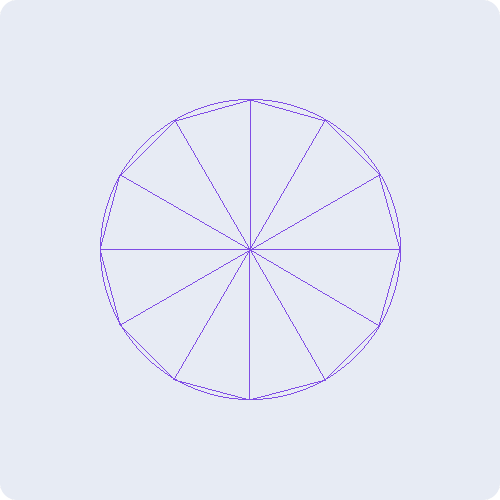
\includegraphics[width=15cm]{src/tarea1.png}\\
\end{center}
\newpage
\Large{\textbf{Algoritmo para encontrar las intersecciones de 5 círculos con centros y radios aleatorios}}\\[0.5cm]
% \section{}
Primero  creamos una lista y guardamos en ella los puntos de los círculos.
\begin{center}
\begin{mycodeboxl}
\begin{lstlisting}
# Declarar lista de todos los puntos que conforman las lineas
puntos8=[]
def circulo8vias(x0, y0, r):
    plot (x0, y0 + r)
    puntos8.append((x0, y0 + r))
    plot (x0, y0 - r)
    puntos8.append((x0, y0 - r))
    plot (x0 + r, y0)
    puntos8.append((x0 + r, y0))
    plot (x0 - r, y0)
    puntos8.append((x0 - r, y0))
    x=1
    y = math.floor(math.sqrt(r * r - x * x) + 0.5)
    while x < y:
        plot(x0 + x, y0 + y)
        puntos8.append((x0 + x, y0 + y))
        plot(x0 + x, y0 - y)
        puntos8.append((x0 + x, y0 - y))
        plot(x0 - x, y0 + y)
        puntos8.append((x0 - x, y0 + y))
        plot(x0 - x, y0 - y)
        puntos8.append((x0 - x, y0 - y))
        plot(x0 + y, y0 + x)
        puntos8.append((x0 + y, y0 + x))
        plot(x0 + y, y0 - x)
        puntos8.append((x0 + y, y0 - x))
        plot(x0 - y, y0 + x)
        puntos8.append((x0 - y, y0 + x))
        plot(x0 - y, y0 - x)
        puntos8.append((x0 - y, y0 - x))
        x = x + 1
        y = math.floor(math.sqrt(r * r - x * x) + 0.5)
\end{lstlisting}
\end{mycodeboxl}
\end{center}
\begin{center}
\begin{mycodeboxl}
\begin{lstlisting}
    if x == y: 
        plot(x0 + x, y0 + y)
        puntos8.append((x0 + x, y0 + y))
        plot(x0 + x, y0 - y)
        puntos8.append((x0 + x, y0 - y))
        plot(x0 - x, y0 + y)
        puntos8.append((x0 - x, y0 + y))
        plot(x0 - x, y0 - y)
        puntos8.append((x0 - x, y0 - y))
\end{lstlisting}
\end{mycodeboxl}
\end{center}

% \newpage
En la función display dibujaremos las 5 lineas requeridas, con valores aleatorios en los puntos.
\begin{center}
\begin{mycodebox}
\begin{lstlisting}
def display():
    glClear(GL_COLOR_BUFFER_BIT)
    glPointSize (1)
    puntos8.clear()
    glColor3f(0.5, 0.3, 0.9) 

    for _ in range(5):
        r = random.randint(50, 100)
        # Para asegurar que los círculos se dibujen dentro de los límites de la ventana 
        x0 = random.randint(r, 499-r)
        y0 = random.randint(r, 499-r)
        circulo8vias(x0, y0, r)
\end{lstlisting}
\end{mycodebox}
\end{center}
    % \includegraphics[width=15cm]{src/pelicula.png}\\
\newpage
Verificaremos los puntos repetidos, en la lista punros8, que serán las intersecciones. 

Dibujaremos puntos de otro color con esas coordenadas para resaltar las intersecciones.
\begin{center}
    
\begin{mycodeboxl}
\begin{lstlisting}
    # Lista para los puntos duplicado (intersección) 
    interseccion = []
    # Crear un conjunto para llevar un registro de los puntos únicos que hemos visto
    puntos_unicos = set()

    # Recorremos la lista de puntos
    for punto in puntos8:
        if punto in puntos_unicos:
            # Si los puntos se encuentran en el conjunto, se añaden a la lista intersección. Inicialmente no hay elementos en el conjunto 
            interseccion.append(punto)
        else:
            # Si no se encuentra el punto en el conjunto, entonces este se añade al mismo conjunto que se utilicará en la próxima iteración
            puntos_unicos.add(punto)
    print("Puntos de intersección de las lineas:", interseccion)

    # Pintar de otro color los puntos de intersección
    glColor3f(0.05, 0.08, 0.1) 
    glPointSize(4)

    # Recorrer la lista de duplicados para dibujarlos 
    for punto in interseccion:
        x, y = punto
        plot(x, y)
    glPointSize(1)
    glFlush()
\end{lstlisting}
\end{mycodeboxl}
\end{center}

\newpage
\Large{\textbf{Capturas de la ventana de gráficos}}\\
\begin{center}
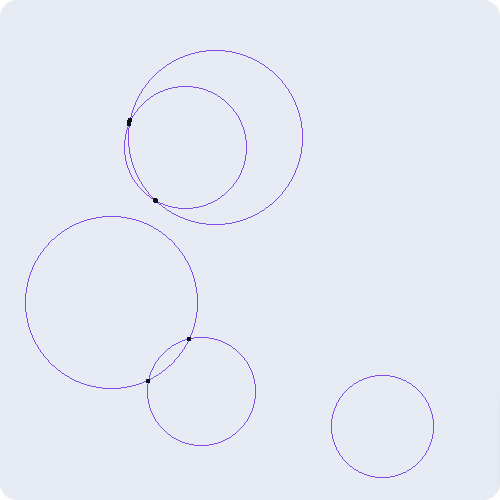
\includegraphics[width=9cm]{src/tarea2_1.png}
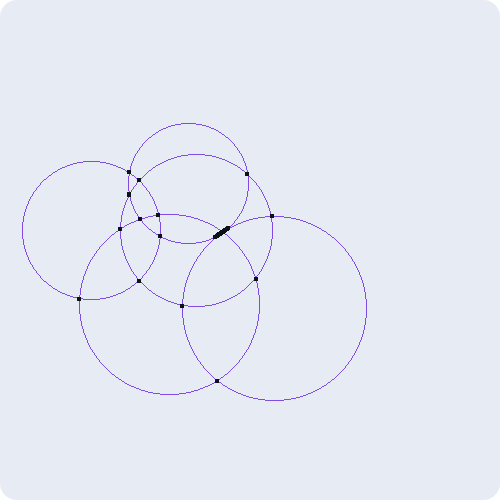
\includegraphics[width=9cm]{src/tarea2_2.png}\\[0.15cm]
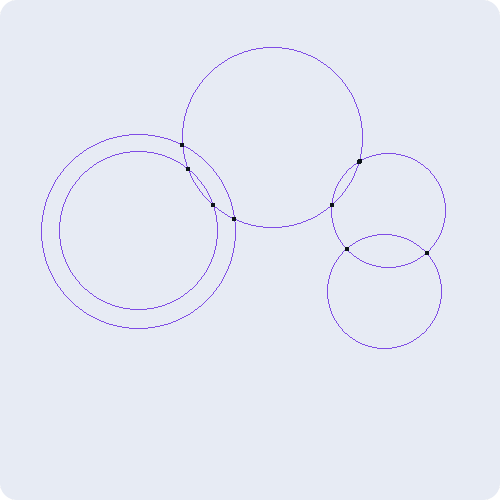
\includegraphics[width=9cm]{src/tarea2_3.png}
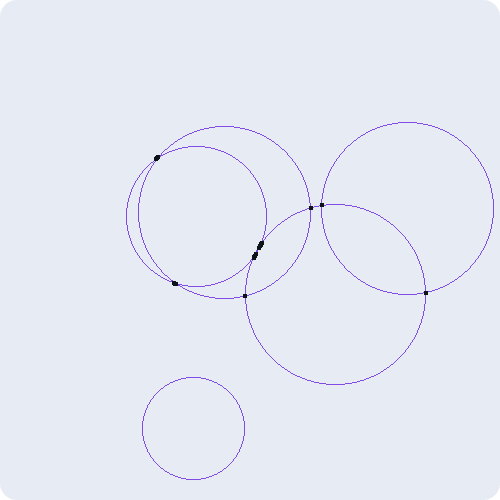
\includegraphics[width=9cm]{src/tarea2_4.png}
\end{center}
\end{document}
